Il servizio Teamwork fornisce un sistema per la gestione dei tasks e creazione delle milestone.
Si è quindi deciso di utilizzare questo servizio.\\

\subsection{Creazione e gestione dei tasks}

I tasks vengo creati e gestiti quasi tutti dal responsabile di progetto.
Qualora il verificatore trovasse imprecisioni od errori trovati durante la verifica avrà la possibilità di creare dei tasks per segnalare suddetti errori.

Ogni tasks può essere assegnato ad uno o più membri del gruppo a seconda della complessità del lavoro e alla disponibilità dei membri del gruppo; i tasks avranno le seguenti caratteristiche:

Per creare un nuovo task bisogna:

\begin{itemize}
	\item Andare su Tasks;
	\item Premere add Task list;
	\item Compilare i campi richiesti;
	\item Aggiungere una task alla task list;
	\item Compilare i campi richiesti.
\end{itemize}
 
\begin{figure}[h]
\centering
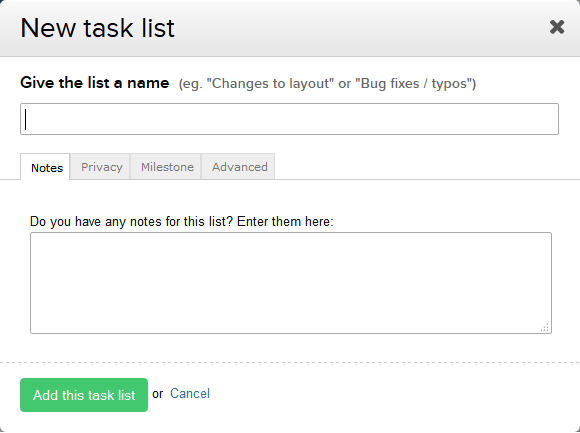
\includegraphics[height= 4cm] {./img/tasklist_fig01.png}
\caption{Creazione task list}

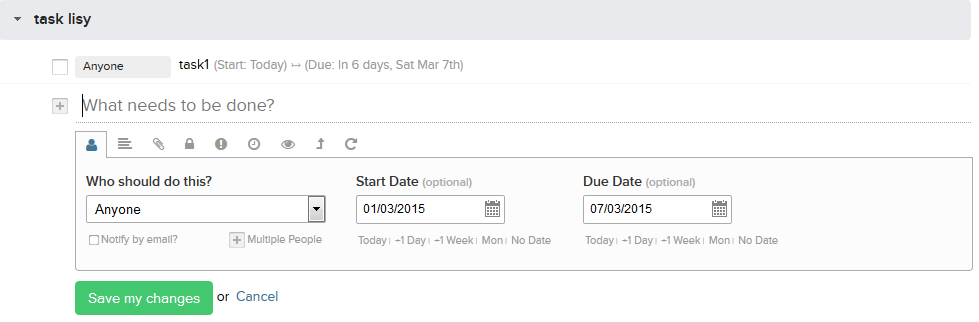
\includegraphics[height= 4cm] {./img/task_fig01.png}
\caption{Creazione task}
\end{figure}

\subsection{Creazione delle milestone}

Il responsabile di progetto ha il compito della creazione di una milestone in occasione di ogni revisione al quale il gruppo DazzleWork ha intenzione di partecipare, più altre milestone qualora il responsabile di progetto lo ritena necessario.

Per creare una nuova milestone bisogna:

\begin{itemize}
	\item Andare su milestone;
	\item Premere add a milesone;
	\item Compilare i campi richiesti.
\end{itemize}

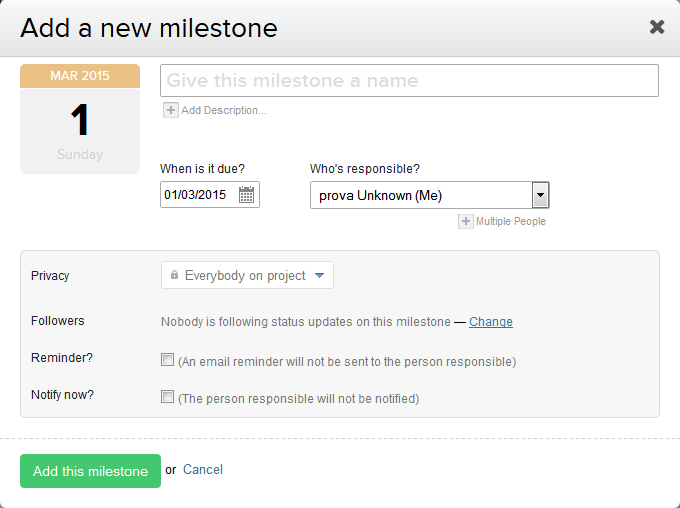
\includegraphics[height= 4cm] {./img/milestone_fig01.png}

\subsection{Esecuzione dei compiti}

Ogni membro del gruppo è tenuto a visionare regolarmente la presenza di tasks a lui assegnati e segnalarne la presa in consegna.
Una volta che un membro porta a termine un task deve modificarne lo stato per segnalare il termine del lavoro.
Se un task scade prima che sia terminato il responsabile di progetto può riaprirlo ed eventualmente assegnare altri membri al lavoro.

\subsection{Chiusura della milestone}

Una volta raggiunta la scadenza, il responsabile di progetto, deve chiudere la milestone ed eventualmente aprirne un'altra per poi ricominciare tutto il protocollo da capo.